\documentclass{article}

\usepackage{listings}
\usepackage{color}
\usepackage{hyperref}
\usepackage{graphicx}
\usepackage{subcaption}
\usepackage{float}

\setlength{\parindent}{0pt}

\renewcommand\lstlistingname{Quelltext} % Change language of section name

\lstset{ % General setup for the package
    language=C,
    basicstyle=\small\sffamily,
    numbers=none,
    %numberstyle=\tiny,
    frame=tb,
    tabsize=4,
    columns=fixed,
    showstringspaces=false,
    showtabs=false,
    keepspaces,
    commentstyle=\color{red},
    keywordstyle=\color{blue}
}

\hypersetup{
    colorlinks=true,
    linkcolor=blue,
    filecolor=magenta,      
    urlcolor=cyan,
}
 
\urlstyle{same}

\title{MCBSTM32C Tutorial}
\author{Claus Holmgaard}
\date{}

\begin{document}

\pagenumbering{gobble}
\maketitle

\newpage
\pagenumbering{arabic}

\section{References}
\href{http://mars.merhot.dk/w/index.php/MCBSTM32C}{Mercantec MCBSTM32C}\\
\href{http://www.st.com/content/ccc/resource/technical/document/datasheet/63/67/d2/6d/88/e0/4e/39/CD00135460.pdf/files/CD00135460.pdf/jcr:content/translations/en.CD00135460.pdf}{LIS302DL Datasheet}\\
\href{http://www.keil.com/pack/doc/CMSIS/Driver/html/group__i2c__interface__gr.html}{Keil CMSIS I2C Driver}\\
\href{http://www.keil.com/dd/docs/datashts/st/stm32f105(7)xx_ds.pdf}{STM32F107VC Datasheet}

\section{New Project}

Create a new project in Keil.
\begin{figure}[H]
    \centering
    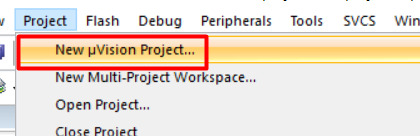
\includegraphics[width=0.8\linewidth]{pics/NewProject.png}
    \caption{New Project.}
    \label{fig:NewProject}
\end{figure}

Choose a place to save it.\\
Then select the device \textit{STM32F107VC}.
\begin{figure}[H]
    \centering
    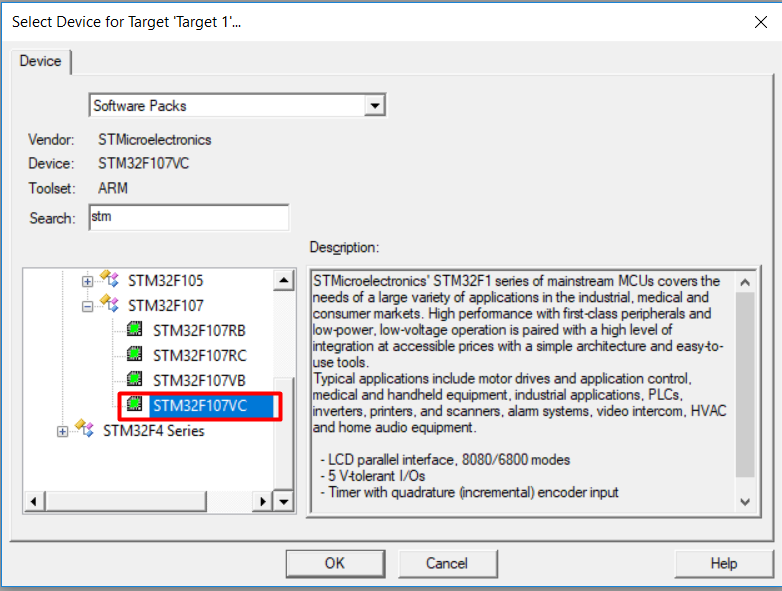
\includegraphics[width=0.8\linewidth]{pics/SelectDevice.png}
    \caption{Select Device.}
    \label{fig:SelectDevice}
\end{figure}

\newpage

The Manage Run-Time Environment should open automatically. If it
does not, open it, and make sure the board variant is \textit{MCBSTM32C}.
It defaults to the E variant.
\begin{figure}[H]
    \centering
    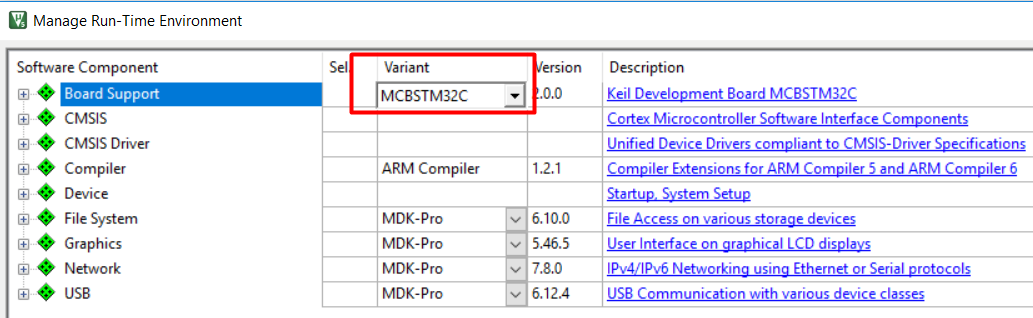
\includegraphics[width=0.8\linewidth]{pics/MRTSetVariant.png}
    \caption{Select Device.}
    \label{fig:SelectDevice}
\end{figure}

Also make sure CMSIS$\to$Core, RTOS$\to$Keil RTX and Device$\to$Startup is selected.
\begin{figure}[H]
    \centering
    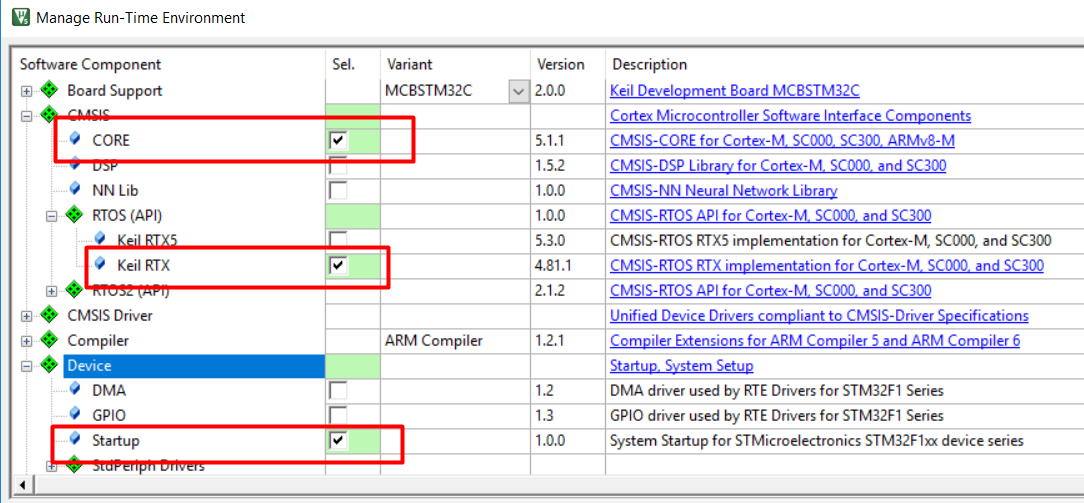
\includegraphics[width=0.8\linewidth]{pics/BasicRuntimeSelection.png}
    \caption{Run time selection.}
    \label{fig:BasicRuntimeSelection}
\end{figure}

Now we want our main .c file, I have called it \textit{tutorial.c}.
In the project pane, expand project, expand the target, then right click the
source group, and select 'Add New Item'. Select a C filetype, and type in the name.
\begin{figure}[H]
    \centering
    \begin{subfigure}[b]{0.45\linewidth}
        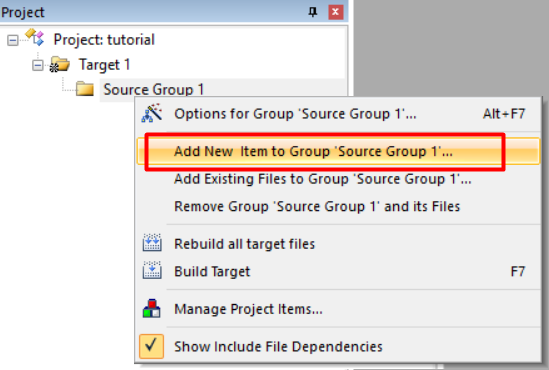
\includegraphics[width=\linewidth]{pics/AddNewFile.png}
        \caption{Add new file.}
    \end{subfigure}
    \begin{subfigure}[b]{0.45\linewidth}
        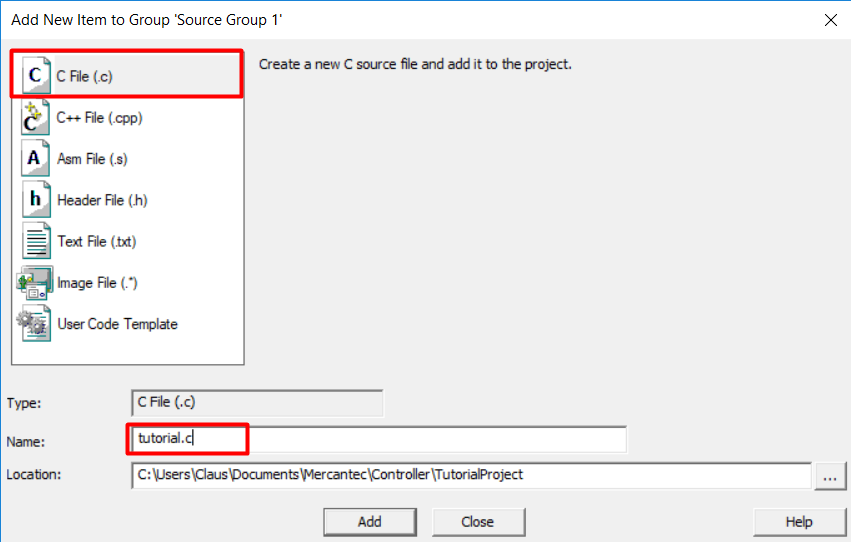
\includegraphics[width=\linewidth]{pics/AddNewFileDialog.png}
        \caption{Type and name.}
    \end{subfigure}
    \label{fig:AddNewFile}
\end{figure}

\newpage

Our project now looks like this, where tutorial.c is empty.
\begin{figure}[H]
    \centering
    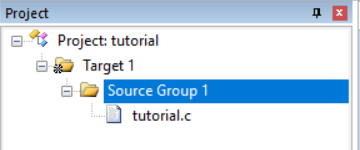
\includegraphics[width=0.5\linewidth]{pics/ProjectStructure1.png}
    \caption{Project Structure.}
    \label{fig:ProjectStructure1}
\end{figure}

We add the most basic code to tutorial.c, and try to compile it.
\begin{figure}[H]
    \centering
    \begin{subfigure}[b]{0.45\linewidth}
        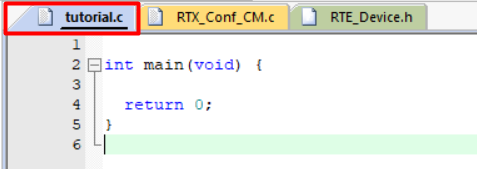
\includegraphics[width=\linewidth]{pics/tutorial_c_basic.png}
        \caption{tutorial.c.}
    \end{subfigure}
    \begin{subfigure}[b]{0.45\linewidth}
        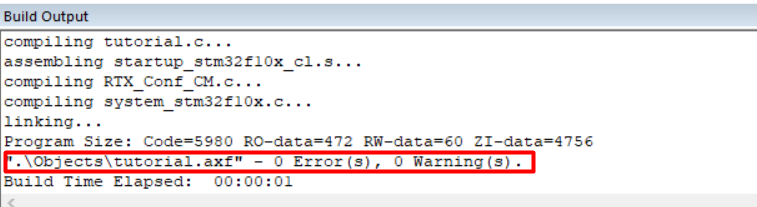
\includegraphics[width=\linewidth]{pics/BasicCompile.png}
        \caption{Compile output.}
    \end{subfigure}
    \label{fig:BasicCode}
\end{figure}

Open Target Options
\begin{figure}[H]
    \centering
    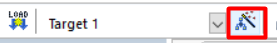
\includegraphics[width=0.5\linewidth]{pics/TargetOptions.png}
    \caption{Target Options.}
    \label{fig:ResetAndRun}
\end{figure}

Open the debug settings, and enable reset and run
\begin{figure}[H]
    \centering
    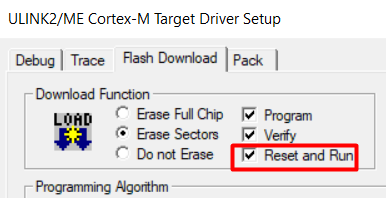
\includegraphics[width=0.5\linewidth]{pics/ResetAndRun.png}
    \caption{Reset and run.}
    \label{fig:ResetAndRun}
\end{figure}

You can load the program on to the chip, though it will do nothing at this point.
\begin{figure}[H]
    \centering
    \begin{subfigure}[b]{0.3\linewidth}
        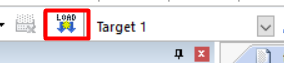
\includegraphics[width=\linewidth]{pics/load.png}
        \caption{Load to device.}
    \end{subfigure}
    \begin{subfigure}[b]{0.6\linewidth}
        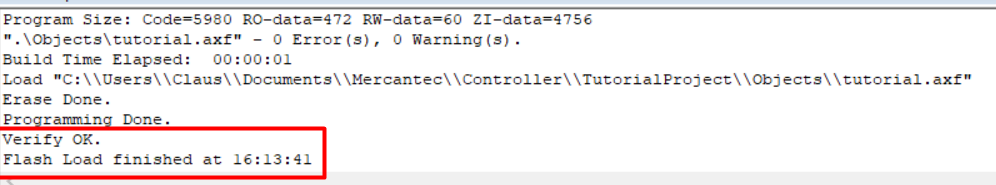
\includegraphics[width=\linewidth]{pics/loadOk.png}
        \caption{Load output.}
    \end{subfigure}
    \label{fig:BasicLoad}
\end{figure}

At this point, the very basic Structure for a project is there, and we're ready
to move on. As someone who's not entirely sure what we're doing, we want debugging output next.

\newpage
\section{Debugging using printf}
First, there's some setup to do.\\
Like before, open the target options. Set the Xtal frequency to 25MHz. Then, also like before,
open the debug settings and set the core clock to 72MHz.
\begin{figure}[H]
    \centering
    \begin{subfigure}[b]{0.45\linewidth}
        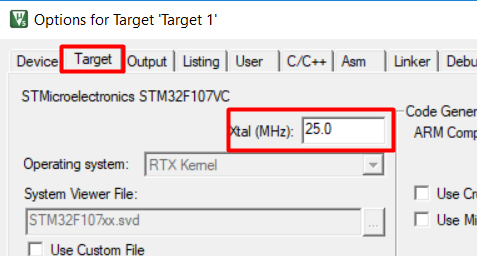
\includegraphics[width=\linewidth]{pics/Xtal.png}
        \caption{Xtal.}
    \end{subfigure}
    \begin{subfigure}[b]{0.45\linewidth}
        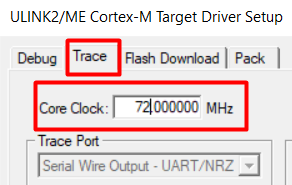
\includegraphics[width=\linewidth]{pics/DebugCoreClock.png}
        \caption{Core clock.}
    \end{subfigure}
    \label{fig:Xtal}
\end{figure}

Open the Run-Time Environment Manager, and make sure \textit{STDERR}, \textit{STDIN}
and \textit{STDOUT} in Compiler$\to$I/O is set to \textit{ITM}.
\begin{figure}[H]
    \centering
    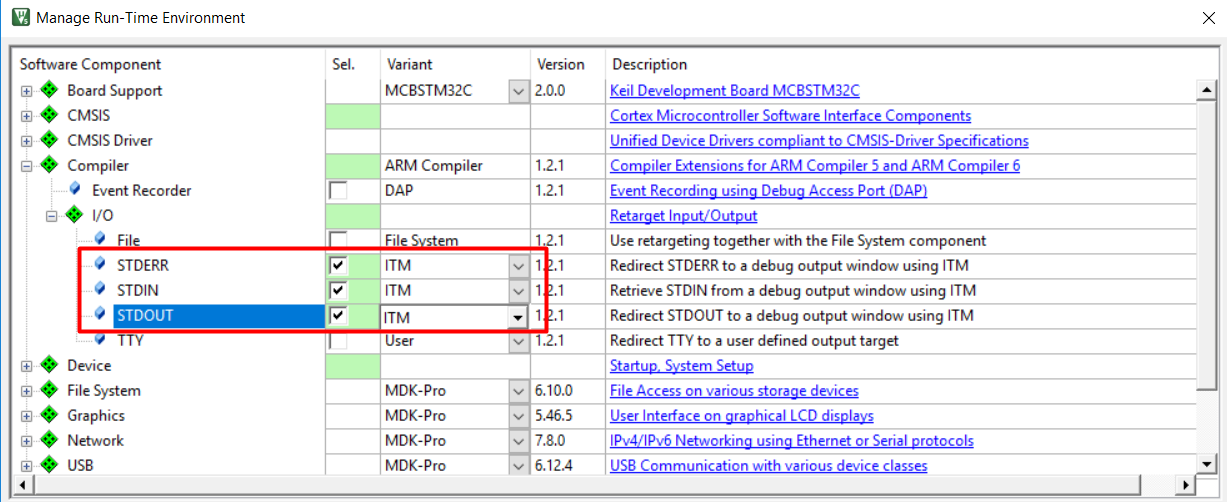
\includegraphics[width=0.8\linewidth]{pics/RuntimeDebug.png}
    \caption{Run time debug settings.}
    \label{fig:Run time debug settings}
\end{figure}

\newpage

In Target Options$\to$Debug$\to$Settings enable Trace, disable timestamps(I found them to generate quite a bit of traffic)
and set the ITM Stimulus Ports.
\begin{figure}[H]
    \centering
    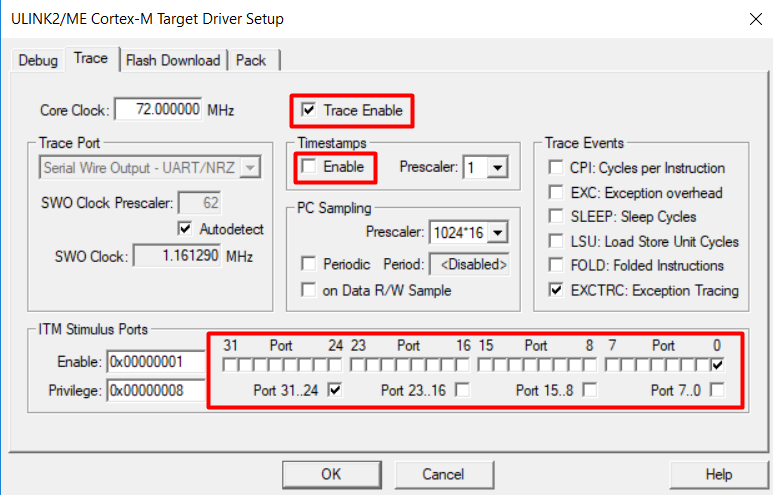
\includegraphics[width=0.8\linewidth]{pics/TraceSetup.png}
    \caption{Trace settings.}
    \label{fig:TraceSettings}
\end{figure}

Apparently printf statements use quite a bit of memory, so we need to increase the stacks size available.
Open the file \textit{CMSIS/RTX\_Conf\_CM.c}, and select the configuration wizard tab.
Here, increase the stacks size.
\begin{figure}[H]
    \centering
    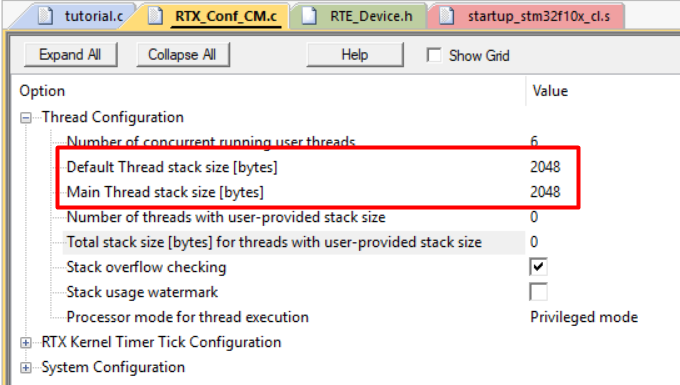
\includegraphics[width=0.8\linewidth]{pics/ThreadStackSize.png}
    \caption{Stacks size.}
    \label{fig:StackSize}
\end{figure}

\newpage

Add a bit more code to \textit{tutorial.c}.\\
We add \textit{stdio.h} to get access to \textit{printf}, and \textit{cmsis\_os.h}
to get access to \textit{osDelay}.
\begin{figure}[H]
    \centering
    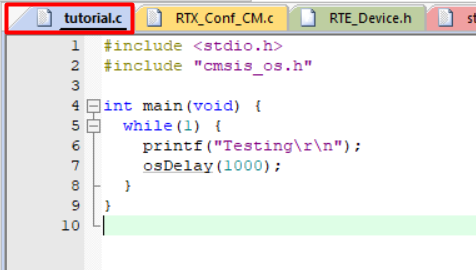
\includegraphics[width=0.8\linewidth]{pics/PrintfMain.png}
    \caption{More code.}
    \label{fig:ModeCode}
\end{figure}

Compile the code, and start the debugger.
\begin{figure}[H]
    \centering
    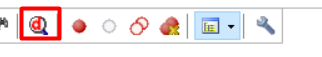
\includegraphics[width=0.5\linewidth]{pics/StartDebugger.png}
    \caption{Start the debugger.}
    \label{fig:StartDebugger}
\end{figure}

\newpage

Open the printf debug viewer.
\begin{figure}[H]
    \centering
    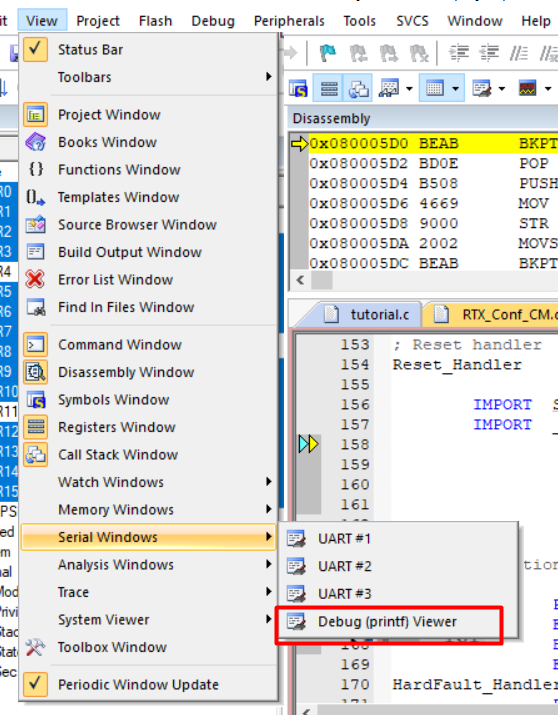
\includegraphics[width=0.8\linewidth]{pics/DebugWindow.png}
    \caption{Debug window.}
    \label{fig:DebugWindow}
\end{figure}

Start the debug session.
\begin{figure}[H]
    \centering
    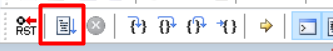
\includegraphics[width=0.5\linewidth]{pics/RunDebugSession.png}
    \caption{Start debug.}
    \label{fig:StartDebugger}
\end{figure}

\newpage

And the output from the printf statement should appear in the debug window.
\begin{figure}[H]
    \centering
    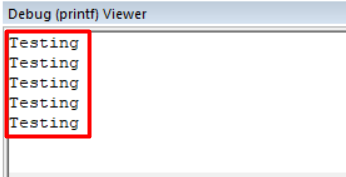
\includegraphics[width=0.5\linewidth]{pics/DebugOutput.png}
    \caption{Debug output.}
    \label{fig:DebugOutput}
\end{figure}

\newpage

\section{LCD}
In order to get the LCD to work, we first add it in the Run-Time Environment Manager,
and click resolve. This will add the LCD, and the SPI drivers.
\begin{figure}[H]
    \centering
    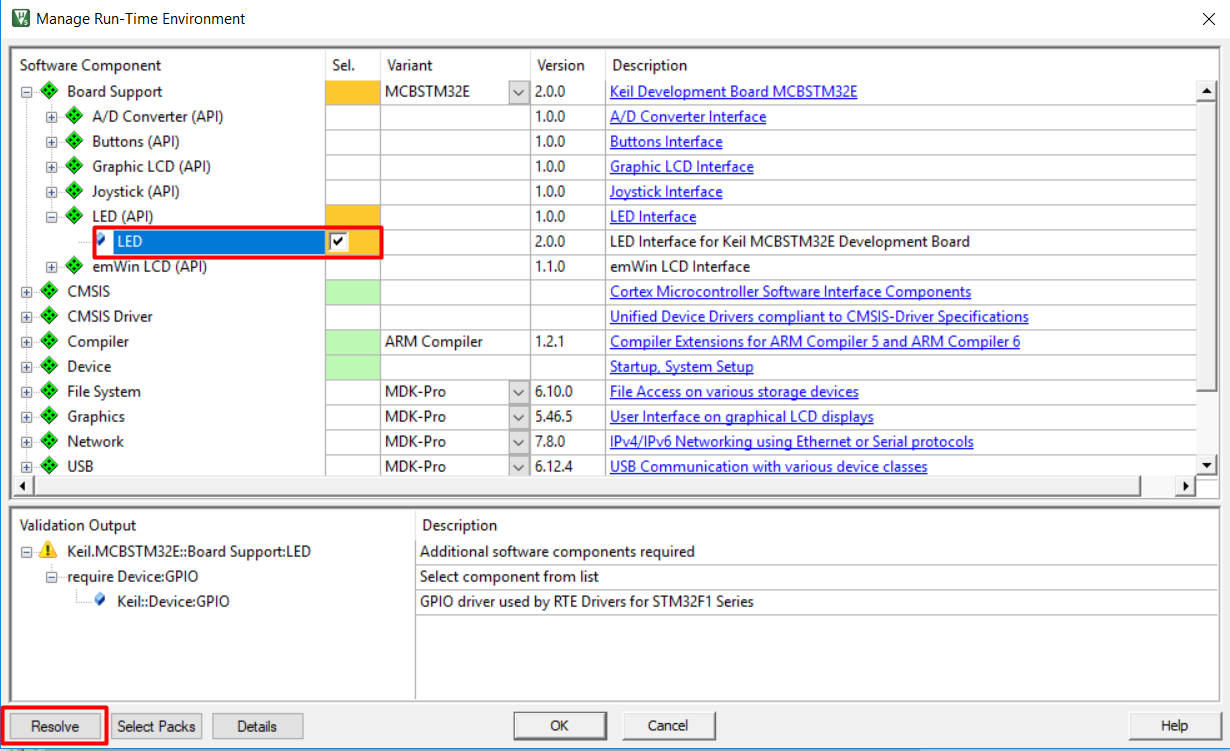
\includegraphics[width=0.8\linewidth]{pics/LEDRuntime.png}
    \caption{LED run-time.}
    \label{fig:LEDRuntime}
\end{figure}

Configure SPI3 in \textit{RTE\_Device.h}.
\begin{figure}[H]
    \centering
    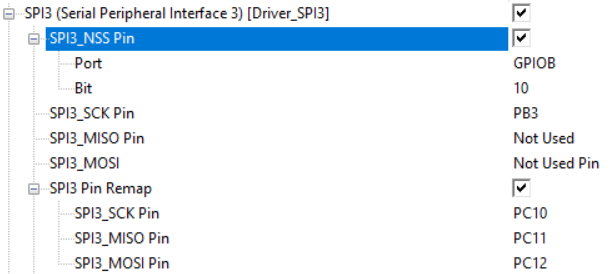
\includegraphics[width=0.8\linewidth]{pics/LCDSPISetup.png}
    \caption{LCD SPI Setup.}
    \label{fig:LCDSPISetup}
\end{figure}

\newpage

I find it useful to keep functionality separated in different files, so
we add MyLCD.h and MyLCD.c to the project, making it look like this.
\begin{figure}[H]
    \centering
    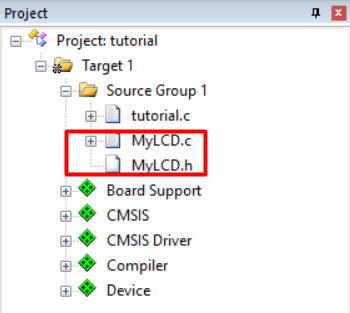
\includegraphics[width=0.4\linewidth]{pics/LCDProject.png}
    \caption{Project with LCD files.}
    \label{fig:LCDProject}
\end{figure}

As the files start getting larger, screenshots of the code will be difficult to work with
(screenshots of code always is, really.) So I will add it here, in a way that you should
be able to copy/paste it.If something isn't clear, the entire project can be found
\href{https://github.com/ClausHolmgaard/MCBSTM32C_Tutorial}{here}, as can this documentation.\\
In \textit{MyLCD.h} we want the following code.

\begin{lstlisting}
    #include <stdio.h>
    #include "cmsis_os.h"
    #include "Board_GLCD.h"
    #include "GLCD_Config.h"

    #ifndef __MY_LCD_H
    #define __MY_LCD_H

    void InitDisplay(void);
    void Display(void);

    #endif
\end{lstlisting}
There's two new include files for the LCD.\\
the \textit{ifndef/define/endif} block is a c preprocessor directive, that makes
sure everything in the block is only included once.\\
\\
In \textit{MyLCD.c} the code is.
\begin{lstlisting}
    #include "MyLCD.h"

    extern GLCD_FONT GLCD_Font_16x24;

    void InitDisplay(void) {
    GLCD_Initialize         ();
    GLCD_SetBackgroundColor (GLCD_COLOR_BLUE);
    GLCD_SetForegroundColor (GLCD_COLOR_WHITE);
    GLCD_ClearScreen        ();
    GLCD_SetFont            (&GLCD_Font_16x24);
    }

    void Display(void) {
        GLCD_DrawString(0, 4*24, "      Hello!      ");
    }
\end{lstlisting}
Note the external variable \textit{GLCD\_FONT}, this initialization sets our
font to 16x24 pixels in size. Furthermore, the background color is set to blue,
foreground color white and the screen is cleared.\\
\\
In \textit{tutorial.c} we can now include \textit{MyLCD.h} and use the functionality
from it.
\begin{lstlisting}
    #include <stdio.h>
    #include "cmsis_os.h"

    #include "MyLCD.h"

    int main(void) {
        
        InitDisplay();
        Display();

        while(1);
    }    
\end{lstlisting}
At this point, it's relevant to mention that the compiler expects every file
end with a newline, if it doesn't you will get a warning during compilation.\\
When this is compiled and flashed, the display should turn on, and display the message "Hello!".

\newpage

\section{I2C \& Accelerometer}
Looking at the \textit{Digital Interfaces} Section of the \href{http://www.st.com/content/ccc/resource/technical/document/datasheet/63/67/d2/6d/88/e0/4e/39/CD00135460.pdf/files/CD00135460.pdf/jcr:content/translations/en.CD00135460.pdf}{LIS302DL datasheet},
we find that it supports SPI and I2C communication. What determines what is used
is the CS pin on the chip, 0 beeing SPI and 1 I2C. On the \href{http://www.keil.com/mcbstm32c/mcbstm32c-base-board-schematics.pdf}{board schematics},
we find the CS pin is set to 3.3V, meaning the pin is high, and I2C communication is used.\\
\begin{figure}[H]
    \centering
    \begin{subfigure}[b]{0.45\linewidth}
        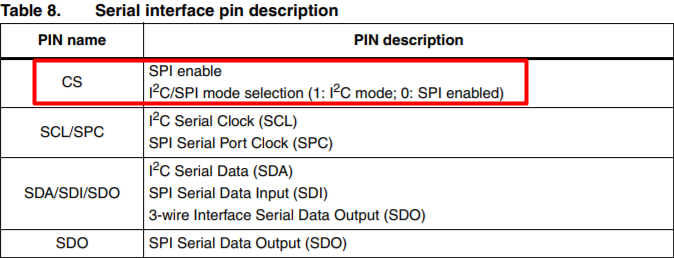
\includegraphics[width=\linewidth]{pics/I2CChipSelect.png}
        \caption{LIS302DL CS.}
    \end{subfigure}
    \begin{subfigure}[b]{0.45\linewidth}
        \includegraphics[width=\linewidth]{pics/LISCSHigh.png}
        \caption{CS on Diagram.}
    \end{subfigure}
    \label{fig:CS}
\end{figure}

First we need to add the I2C driver to the Run-Time Environment.
\begin{figure}[H]
    \centering
    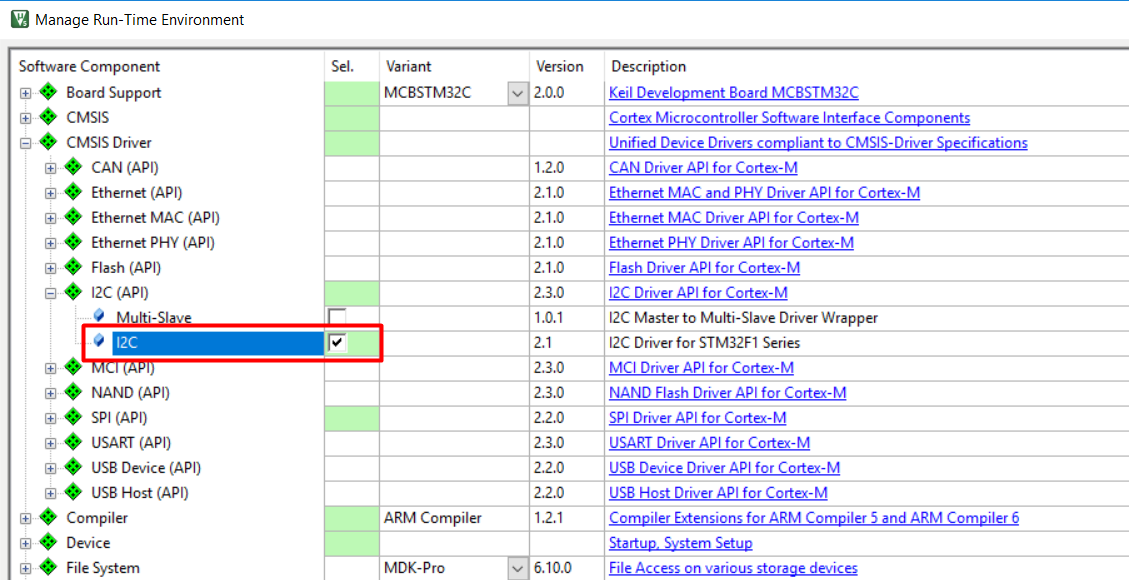
\includegraphics[width=0.8\linewidth]{pics/I2CRuntime.png}
    \caption{I2C Run-Time Settings.}
    \label{fig:I2CRuntime}
\end{figure}

In the \href{http://www.keil.com/mcbstm32c/mcbstm32c-base-board-schematics.pdf}{board schematics}
we can see the Accelerometer chip is connected to PB8 and 9 on the STM32F107 chip.
Looking in the \href{http://www.keil.com/dd/docs/datashts/st/stm32f105(7)xx_ds.pdf}{datasheet},
we can see that these are connected to I2C bus 1.
\begin{figure}[H]
    \centering
    \begin{subfigure}[b]{0.45\linewidth}
        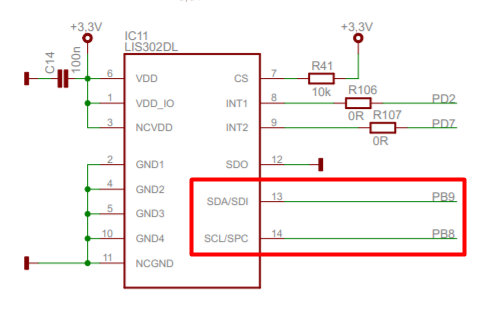
\includegraphics[width=\linewidth]{pics/I2CPinsDiagram.png}
        \caption{LIS302DL I2C Pins.}
    \end{subfigure}
    \begin{subfigure}[b]{0.45\linewidth}
        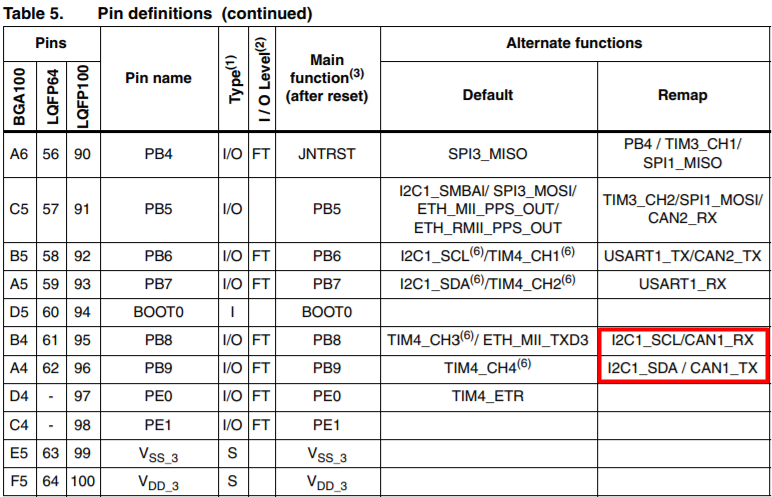
\includegraphics[width=\linewidth]{pics/PB89I2C1.png}
        \caption{I2C Bus.}
    \end{subfigure}
    \label{fig:I2CSettings}
\end{figure}

This can be setup in \textit{RTE\_Device.h}.
\begin{figure}[H]
    \centering
    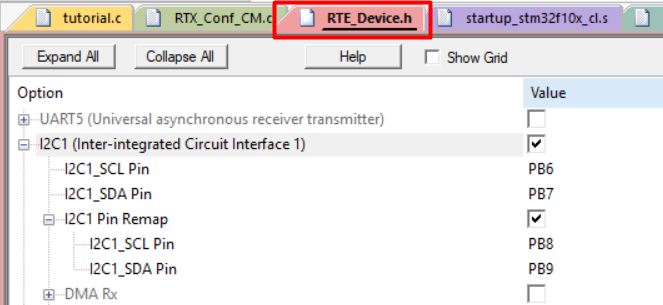
\includegraphics[width=0.8\linewidth]{pics/I2CConfig.png}
    \caption{I2C Config.}
    \label{fig:I2CConfig}
\end{figure}

Now let's add \textit{MyAccelerometer.h} and \textit{MyAccelerometer.c} to the project.
In a larger project I would probably keep the accelerometer code, and the I2C code in seperate files,
but that is unnecessary here.

\newpage

Our project now looks like this.
\begin{figure}[H]
    \centering
    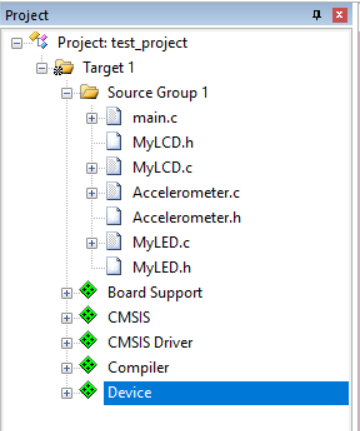
\includegraphics[width=0.35\linewidth]{pics/AccProject.png}
    \caption{Accelerometer Project.}
    \label{fig:AccProject}
\end{figure}

There's quite a bit of code needed to make this work. I'll list it all here,
and go through it after.\\
\\
\textit{MyAccelerometer.h}
\begin{lstlisting}
#include <stdio.h>
#include "Driver_I2C.h"
#include "cmsis_os.h"

#ifndef __ACCELEROMETER_H
#define __ACCELEROMETER_H

typedef struct _ACCELEROMETER_STATE {
int8_t x;
int8_t y;
int8_t z;
} ACCELEROMETER_STATE;

#define ACCELEROMETER_ADDR 			0x1C

#define CTRL_REG1             	0x20
#define OUT_X                 	0x29
#define OUT_Y                 	0x2B
#define OUT_Z                 	0x2D

#ifndef ACCELEROMETER_I2C_PORT
#define ACCELEROMETER_I2C_PORT 	1
#endif

#define _I2C_Driver_(n)  Driver_I2C##n
#define  I2C_Driver_(n)  _I2C_Driver_(n)
extern ARM_DRIVER_I2C    I2C_Driver_(ACCELEROMETER_I2C_PORT);
#define ptrI2C           (&I2C_Driver_(ACCELEROMETER_I2C_PORT))

void I2C_Initialize (void);
int32_t I2C_ReadBuf (uint32_t addr, uint8_t *buf, uint32_t len);
int32_t I2C_WriteBuf (uint8_t reg, uint8_t val);
int32_t Accelerometer_GetState (ACCELEROMETER_STATE *pState);
void I2CHandler(void const *arg);

#endif
\end{lstlisting}

\vspace{2mm}
\textit{MyAccelerometer.c}
\begin{lstlisting}
#include "MyAccelerometer.h"

void I2C_Initialize(void) {
    ptrI2C->Initialize(NULL);
    ptrI2C->PowerControl(ARM_POWER_FULL);
    ptrI2C->Control(ARM_I2C_BUS_SPEED, ARM_I2C_BUS_SPEED_FAST);
    ptrI2C->Control(ARM_I2C_BUS_CLEAR, 0);

    I2C_WriteBuf(CTRL_REG1, 0x47);
    }

    int32_t I2C_WriteBuf (uint8_t reg, uint8_t val) {
    uint8_t data[2];

    data[0] = reg;
    data[1] = val;
    ptrI2C->MasterTransmit(ACCELEROMETER_ADDR, data, 2, false);
    while (ptrI2C->GetStatus().busy);
    if (ptrI2C->GetDataCount() != 2) return -1;

    return 0;
}

int32_t I2C_ReadBuf (uint32_t addr, uint8_t *buf, uint32_t len) {
    uint8_t a[1];
    
    uint32_t I2CAddr = ACCELEROMETER_ADDR;
    
    int32_t transmit_request_status;
    int32_t transmit2_receive_status;
    int32_t data_count;
    
    a[0] = (uint8_t)addr;
    
    transmit_request_status = ptrI2C->MasterTransmit(I2CAddr, a, 1, true);
    if(transmit_request_status != 0) {
        return -1;
    }

    while(ptrI2C->GetStatus().busy);
    transmit2_receive_status = ptrI2C->MasterReceive(I2CAddr, buf, len, false);
    if(transmit2_receive_status != 0) {
        return -1;
    }

    while(ptrI2C->GetStatus().busy);
    data_count = ptrI2C->GetDataCount();
    if(data_count != len) {
        return -1;
    }

return 0;
}

int32_t Accelerometer_GetState (ACCELEROMETER_STATE *pState) {
    uint8_t val;

    int8_t x;
    int8_t y;
    int8_t z;
        
    I2C_ReadBuf(OUT_X, &val, 1);
    x = (int8_t)val;

    I2C_ReadBuf(OUT_Y, &val, 1);
    y = (int8_t)val;

    I2C_ReadBuf(OUT_Z, &val, 1);
    z = (int8_t)val;

    pState->x = x;
    pState->y = y;
    pState->z = z;
        
    return 0;
}

void I2CHandler(void const *arg) {
    uint8_t val;
    uint32_t rec_status;
    ACCELEROMETER_STATE acc;

    rec_status = I2C_ReadBuf(0x0F, &val, 1);
    printf("Receive status: %d\r\n", rec_status);
    printf("Val: 0x%02X\r\n", val);
    
    while(1) {
        Accelerometer_GetState(&acc);
        printf("Acc X = %d\r\n", acc.x);
        printf("Acc Y = %d\r\n", acc.y);
        printf("Acc Z = %d\r\n", acc.z);
        printf("\r\n");
        
        osDelay(100);
    }
}
\end{lstlisting}

\vspace{2mm}
\textit{main.c}
\begin{lstlisting}
    #include <stdio.h>
    #include "cmsis_os.h"

    #include "MyLCD.h"
    #include "MyAccelerometer.h"

    osThreadId TID_Accelerometer;

    osThreadDef(I2CHandler, osPriorityNormal, 1, 0);

    int main(void) {
        
        InitDisplay();
        I2C_Initialize();
        
        Display();
        
        TID_Accelerometer = osThreadCreate(osThread(I2CHandler), NULL);
        
        while(1);
    }
\end{lstlisting}

\vspace{2mm}
Starting with \textit{MyAccelerometer.h}.\\
The first new thing is the definition of \textit{\_ACCELEROMETER\_STATE}, it's
used as a convenience when getting the state of the accelerometer.

\end{document}
